\documentclass[hyperref={pdfpagelabels=false}]{beamer}

\usepackage{focs-poster}
\usetikzlibrary{arrows.meta,positioning}

\definecolor{posterink}{HTML}{173A38}
\definecolor{posterteal}{HTML}{236B65}
\definecolor{posterblue}{HTML}{3E7198}
\definecolor{posterpurple}{HTML}{76689A}
\definecolor{postergold}{HTML}{C98B38}
\definecolor{posterpaper}{HTML}{F4F0E8}
\definecolor{postermuted}{HTML}{5F6C69}

\setbeamercolor{normal text}{fg=posterink,bg=posterpaper}
\setbeamercolor{structure}{fg=posterteal}
\setbeamercolor{itemize item}{fg=posterteal}

\newtcolorbox{musicpanel}[2][]{
  enhanced,
  colback=white,
  opacityback=.80,
  colframe=#2!55!posterink,
  opacityframe=.82,
  boxrule=.72mm,
  arc=4mm,
  left=.78cm,
  right=.78cm,
  top=.66cm,
  bottom=.66cm,
  fontupper=\fontsize{29}{35}\selectfont,
  overlay={
    \draw[#2,line width=1.35mm,line cap=round]
      ([xshift=.9cm]frame.north west) -- ([xshift=8.4cm]frame.north west);
    \draw[#2!85!posterink,line width=.72mm,line cap=round,line join=round]
      ([xshift=-8.0cm]frame.north east)
      -- ++(.75cm,0) -- ++(.30cm,.28cm) -- ++(.38cm,-.56cm)
      -- ++(.42cm,.84cm) -- ++(.46cm,-1.12cm) -- ++(.42cm,.84cm)
      -- ++(.38cm,-.56cm) -- ++(.30cm,.28cm) -- ++(.75cm,0);
    \begin{scope}
      \clip (interior.south west) rectangle (interior.north east);
      \coordinate (groove) at ([xshift=-.15cm,yshift=.15cm]interior.south east);
      \draw[#2,opacity=.12,line width=.65mm] (groove) circle (1.55cm);
      \draw[#2,opacity=.12,line width=.65mm] (groove) circle (2.45cm);
      \draw[#2,opacity=.12,line width=.65mm] (groove) circle (3.35cm);
      \fill[#2,opacity=.15] (groove) circle (.28cm);
    \end{scope}
  },
  #1
}

\tcbset{
  narrativecard/.style={
    enhanced,
    colback=white,
    opacityback=.34,
    opacityframe=0,
    boxrule=1.45mm,
    arc=7mm,
    left=.88cm,
    right=.88cm,
    top=.78cm,
    bottom=.78cm,
    fontupper=\fontsize{31}{37}\selectfont
  },
  evidencecard/.style={
    enhanced,
    colback=white,
    opacityback=.24,
    opacityframe=0,
    boxrule=1.55mm,
    arc=1.8mm,
    left=.88cm,
    right=.88cm,
    top=.78cm,
    bottom=.78cm,
    fontupper=\fontsize{31}{37}\selectfont
  }
}

\newtcolorbox{targetcard}[1][]{
  narrativecard,
  colframe=posterteal!76!posterink,
  borderline={5.0mm}{0mm}{posterteal!12!white},
  borderline={1.45mm}{0mm}{posterteal!82!posterink},
  borderline={.34mm}{-1.25mm}{white!88!posterteal},
  overlay={
    \draw[posterteal!94!posterink,line width=3.6mm,line cap=round]
      ([xshift=.85cm]frame.north west) -- ([xshift=8.2cm]frame.north west);
    \draw[posterteal!94!posterink,line width=3.6mm,line cap=round]
      ([yshift=-.85cm]frame.north west) -- ([yshift=-8.1cm]frame.north west);
    \draw[posterteal!92!posterink,line width=1.45mm,line cap=round,line join=round]
      ([xshift=-9.7cm]frame.north east)
      -- ++(.85cm,0) -- ++(.30cm,.42cm) -- ++(.36cm,-.84cm)
      -- ++(.42cm,1.26cm) -- ++(.46cm,-1.68cm) -- ++(.42cm,1.26cm)
      -- ++(.36cm,-.84cm) -- ++(.30cm,.42cm) -- ++(.85cm,0);
    \foreach \dy in {-5.0,-9.0,-13.0}{
      \draw[posterteal!90!posterink,line width=1.35mm,line cap=round]
        ([xshift=-.58cm,yshift=\dy cm]frame.north east)
        -- ([xshift=.72cm,yshift=\dy cm]frame.north east);
      \fill[posterteal!92!posterink]
        ([yshift=\dy cm]frame.north east) circle (.22cm);
    }
  },
  #1
}

\newtcolorbox{investmentcard}[1][]{
  narrativecard,
  colframe=postergold!82!posterink,
  borderline={5.0mm}{0mm}{postergold!14!white},
  borderline={1.45mm}{0mm}{postergold!86!posterink},
  borderline={.34mm}{-1.25mm}{white!88!postergold},
  overlay={
    \draw[postergold!94!black,line width=3.6mm,line cap=round]
      ([xshift=.85cm]frame.north west) -- ([xshift=8.2cm]frame.north west);
    \draw[postergold!94!black,line width=3.6mm,line cap=round]
      ([yshift=-.85cm]frame.north west) -- ([yshift=-7.8cm]frame.north west);
    \draw[-{Latex[length=4.2mm,width=3.0mm]},postergold!90!black,
      line width=1.42mm,line cap=round,line join=round]
      ([xshift=2.5cm,yshift=-1.10cm]frame.south west)
      -- ++(4.0cm,0) -- ++(0,.42cm) -- ++(4.0cm,0)
      -- ++(0,.43cm) -- ++(4.0cm,0) -- ++(0,.44cm) -- ++(4.8cm,0);
    \foreach \x in {3.2,7.2,11.2,15.2}{
      \draw[postergold!82!posterink,line width=1.05mm]
        ([xshift=\x cm,yshift=-.28cm]frame.south west)
        -- ([xshift=\x cm,yshift=.28cm]frame.south west);
    }
  },
  #1
}

\newtcolorbox{discoverycard}[1][]{
  evidencecard,
  colframe=posterpurple!78!posterink,
  borderline={4.4mm}{0mm}{posterpurple!13!white},
  borderline={1.55mm}{0mm}{posterpurple!84!posterink},
  borderline={.38mm}{-1.30mm}{white!88!posterpurple},
  overlay={
    \draw[posterpurple!95!posterink,line width=3.15mm,line cap=round]
      ([xshift=.72cm]frame.north west) -- ([xshift=7.8cm]frame.north west);
    \foreach \dy in {-.34,-.17,0,.17,.34}{
      \draw[posterpurple!70!posterink,line width=.52mm,line cap=round]
        ([xshift=-11.7cm,yshift=\dy cm]frame.north east)
        -- ([xshift=-.75cm,yshift=\dy cm]frame.north east);
    }
    \coordinate (discoverRoot) at ([xshift=-10.6cm]frame.north east);
    \coordinate (discoverUpper) at ([xshift=-7.8cm,yshift=.52cm]frame.north east);
    \coordinate (discoverMiddle) at ([xshift=-7.5cm]frame.north east);
    \coordinate (discoverLower) at ([xshift=-7.8cm,yshift=-.52cm]frame.north east);
    \coordinate (discoverMerge) at ([xshift=-3.5cm]frame.north east);
    \draw[posterpurple!94!posterink,line width=1.40mm,line cap=round]
      (discoverRoot) -- (discoverUpper) -- (discoverMerge)
      (discoverRoot) -- (discoverMiddle) -- (discoverMerge)
      (discoverRoot) -- (discoverLower) -- (discoverMerge);
    \foreach \p in {discoverRoot,discoverUpper,discoverMiddle,discoverLower,discoverMerge}
      \fill[posterpurple!94!posterink] (\p) circle (.22cm);
    \foreach \dy in {-5.0,-9.0,-13.0}{
      \fill[posterpurple!86!posterink]
        ([yshift=\dy cm]frame.north east) circle (.20cm);
    }
  },
  #1
}

\newtcolorbox{graphcard}[1][]{
  evidencecard,
  colframe=posterpurple!78!posterink,
  borderline={4.4mm}{0mm}{posterpurple!13!white},
  borderline={1.55mm}{0mm}{posterpurple!84!posterink},
  borderline={.38mm}{-1.30mm}{white!88!posterpurple},
  overlay={
    \draw[posterpurple!95!posterink,line width=3.15mm,line cap=round]
      ([xshift=.72cm]frame.north west) -- ([xshift=7.8cm]frame.north west);
    \draw[posterpurple!90!posterink,line width=1.34mm,line cap=round]
      ([xshift=1.7cm,yshift=.56cm]frame.south west) -- ++(8.6cm,0)
      -- ++(3.0cm,-.56cm) -- ++(7.0cm,0);
    \draw[posterpurple!90!posterink,line width=1.34mm,line cap=round]
      ([xshift=1.7cm]frame.south west) -- ++(19.2cm,0);
    \draw[posterpurple!90!posterink,line width=1.34mm,line cap=round]
      ([xshift=1.7cm,yshift=-.56cm]frame.south west) -- ++(8.6cm,0)
      -- ++(3.0cm,.56cm) -- ++(7.0cm,0);
    \foreach \x/\y in {4.2/.56,7.4/0,10.3/.56,13.3/0,17.0/0,20.0/0}{
      \fill[posterpurple!95!posterink]
        ([xshift=\x cm,yshift=\y cm]frame.south west) circle (.20cm);
    }
    \draw[posterpurple!82!posterink,line width=1.15mm]
      ([yshift=-4.0cm]frame.north east)
      -- ([xshift=-.65cm,yshift=-7.0cm]frame.north east)
      -- ([yshift=-10.0cm]frame.north east)
      -- ([xshift=-.65cm,yshift=-13.0cm]frame.north east);
    \foreach \dy in {-4.0,-10.0}{
      \fill[posterpurple!94!posterink]
        ([yshift=\dy cm]frame.north east) circle (.20cm);
    }
  },
  #1
}

\newtcolorbox{eracard}[1][]{
  evidencecard,
  colframe=posterpurple!78!posterink,
  borderline={4.4mm}{0mm}{posterpurple!13!white},
  borderline={1.55mm}{0mm}{posterpurple!84!posterink},
  borderline={.38mm}{-1.30mm}{white!88!posterpurple},
  overlay={
    \draw[posterpurple!95!posterink,line width=3.15mm,line cap=round]
      ([xshift=.72cm]frame.north west) -- ([xshift=8.4cm]frame.north west);
    \draw[posterpurple!92!posterink,line width=1.35mm,line cap=round]
      ([xshift=1.5cm]frame.south west) -- ([xshift=-4.0cm]frame.south east);
    \foreach \f in {.08,.18,.28,.38,.48,.58,.68,.78,.88}{
      \draw[posterpurple!90!posterink,line width=1.05mm]
        ($(frame.south west)!\f!(frame.south east)+(0,-.46cm)$)
        -- ($(frame.south west)!\f!(frame.south east)+(0,.46cm)$);
    }
    \draw[posterpurple!92!posterink,line width=1.38mm,line cap=round,line join=round]
      ([xshift=-15.0cm]frame.north east)
      -- ++(1.1cm,0) -- ++(.45cm,.42cm) -- ++(.52cm,-.84cm)
      -- ++(.58cm,1.26cm) -- ++(.64cm,-1.68cm) -- ++(.58cm,1.26cm)
      -- ++(.52cm,-.84cm) -- ++(.45cm,.42cm) -- ++(1.1cm,0);
    \foreach \dy in {-4.0,-7.2,-10.4,-13.6}{
      \draw[posterpurple!78!posterink,line width=1.2mm]
        ([xshift=-.54cm,yshift=\dy cm]frame.north east)
        -- ([xshift=.54cm,yshift=\dy cm]frame.north east);
    }
  },
  #1
}

\newcommand{\sectiontitle}[1]{%
  {\fontsize{44}{49}\selectfont\bfseries\color{posterink}#1\par}%
}

\newcommand{\targetmark}{%
  
\begin{tikzpicture}[x=1cm,y=1cm]
    \useasboundingbox (0,-.15) rectangle (24.7,3.45);
    \node[anchor=west,text=posterteal!92!posterink,
      font=\fontsize{22}{24}\selectfont\bfseries] at (0,2.72) {OUR};
    \node[anchor=west,text=posterink,
      font=\fontsize{54}{56}\selectfont\bfseries] at (0,1.08) {TARGET};
    \draw[posterteal!88!posterink,line width=1.25mm,line cap=round]
      (9.0,1.02) -- (21.3,1.02);
    \fill[posterteal!92!posterink] (9.0,1.02) circle (.18cm);
    \draw[-{Latex[length=5mm,width=3.5mm]},posterteal!92!posterink,
      line width=1.25mm,line cap=round] (18.8,1.02) -- (22.6,1.02);
    \draw[posterteal!88!posterink,line width=.86mm,line cap=round]
      (14.4,1.02) -- ++(.35,.40) -- ++(.42,-.80)
      -- ++(.50,1.20) -- ++(.58,-1.60) -- ++(.50,1.20)
      -- ++(.42,-.80) -- ++(.35,.40);
  \end{tikzpicture}%
}

\newcommand{\discoverymark}{%
  
\begin{tikzpicture}[x=1cm,y=1cm]
    \useasboundingbox (0,-.15) rectangle (24.7,3.65);
    \node[anchor=west,text=posterpurple!92!posterink,
      font=\fontsize{22}{24}\selectfont\bfseries] at (0,2.90) {BETTER};
    \node[anchor=west,text=posterink,
      font=\fontsize{50}{52}\selectfont\bfseries] at (0,1.28) {DISCOVERY};
    \coordinate (titleRoot) at (12.4,.42);
    \coordinate (titleUpper) at (16.0,.88);
    \coordinate (titleMiddle) at (16.2,.42);
    \coordinate (titleLower) at (16.0,-.04);
    \coordinate (titleMerge) at (20.2,.42);
    \draw[posterpurple!90!posterink,line width=1.05mm,line cap=round]
      (10.5,.42) -- (titleRoot)
      (titleRoot) -- (titleUpper) -- (titleMerge)
      (titleRoot) -- (titleMiddle) -- (titleMerge)
      (titleRoot) -- (titleLower) -- (titleMerge) -- (23.0,.42);
    \foreach \p in {titleRoot,titleUpper,titleMiddle,titleLower,titleMerge}
      \fill[posterpurple!94!posterink] (\p) circle (.16cm);
  \end{tikzpicture}%
}

\newcommand{\graphmark}{%
  
\begin{tikzpicture}[x=1cm,y=1cm]
    \useasboundingbox (0,-.15) rectangle (24.7,3.65);
    \node[anchor=west,text=posterpurple!94!posterink,
      font=\fontsize{22}{24}\selectfont\bfseries] at (0,2.90) {FASTER};
    \node[anchor=west,text=posterink,
      font=\fontsize{43}{45}\selectfont\bfseries] at (0,1.32) {GRAPH};
    \node[anchor=west,text=posterpurple!88!posterink,
      font=\fontsize{29}{32}\selectfont\bfseries] at (8.7,1.28) {INTELLIGENCE};
    \coordinate (g1) at (1.0,.34);
    \coordinate (g2) at (5.0,.68);
    \coordinate (g3) at (8.4,.18);
    \coordinate (g4) at (12.6,.72);
    \coordinate (g5) at (17.0,.32);
    \coordinate (g6) at (22.8,.56);
    \draw[posterpurple!86!posterink,line width=1.02mm,line cap=round]
      (g1) -- (g2) -- (g4) -- (g6)
      (g1) -- (g3) -- (g4)
      (g3) -- (g5) -- (g6);
    \foreach \p/\r in {g1/.14,g2/.18,g3/.15,g4/.22,g5/.17,g6/.20}
      \fill[posterpurple!94!posterink] (\p) circle (\r cm);
  \end{tikzpicture}%
}

\newcommand{\investmentmark}{%
  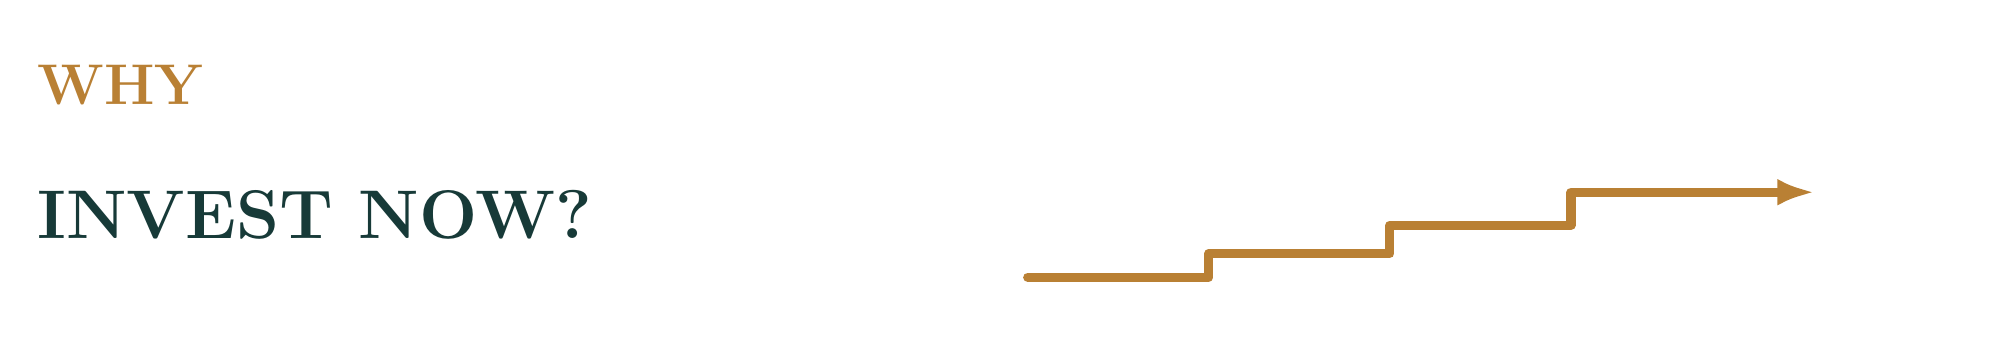
\begin{tikzpicture}[x=1cm,y=1cm]
    \useasboundingbox (0,-.15) rectangle (24.7,3.45);
    \node[anchor=west,text=postergold!92!black,
      font=\fontsize{22}{24}\selectfont\bfseries] at (0,2.72) {WHY};
    \node[anchor=west,text=posterink,
      font=\fontsize{48}{50}\selectfont\bfseries] at (0,1.08) {INVEST NOW?};
    \draw[-{Latex[length=4.8mm,width=3.4mm]},postergold!92!black,
      line width=1.16mm,line cap=round,line join=round]
      (12.7,.28) -- (15.0,.28) -- (15.0,.58) -- (17.3,.58)
      -- (17.3,.94) -- (19.6,.94) -- (19.6,1.36) -- (22.7,1.36);
  \end{tikzpicture}%
}

\newcommand{\eramark}{%
  
\begin{tikzpicture}[x=1cm,y=1cm]
    \useasboundingbox (0,-.15) rectangle (55.0,3.45);
    \node[anchor=west,text=posterpurple!92!posterink,
      font=\fontsize{22}{24}\selectfont\bfseries] at (0,2.72) {SHARPER};
    \node[anchor=west,text=posterink,
      font=\fontsize{52}{54}\selectfont\bfseries] at (0,1.08) {ERA ESTIMATION};
    \draw[posterpurple!90!posterink,line width=1.18mm,line cap=round]
      (22.0,.58) -- (50.8,.58);
    \foreach \x in {23.0,27.0,31.0,35.0,39.0,43.0,47.0,50.0}{
      \draw[posterpurple!88!posterink,line width=.86mm]
        (\x,.20) -- (\x,.96);
    }
    \node[anchor=north,text=postermuted,
      font=\fontsize{20}{23}\selectfont\bfseries] at (23.0,.08) {1920s};
    \node[anchor=north,text=postermuted,
      font=\fontsize{20}{23}\selectfont\bfseries] at (35.0,.08) {1960s};
    \node[anchor=north,text=postermuted,
      font=\fontsize{20}{23}\selectfont\bfseries] at (47.0,.08) {2000s};
    \draw[posterpurple!92!posterink,line width=.92mm,line cap=round,line join=round]
      (37.4,1.48) -- ++(.60,0) -- ++(.24,.30) -- ++(.30,-.60)
      -- ++(.36,.90) -- ++(.42,-1.20) -- ++(.36,.90)
      -- ++(.30,-.60) -- ++(.24,.30) -- ++(.60,0);
  \end{tikzpicture}%
}

\newcommand{\smallnote}[1]{%
  {\fontsize{25}{30}\selectfont\color{postermuted}#1\par}%
}

\newcommand{\yearbar}[4]{%
  \node[anchor=east,font=\bfseries] at (0,#1+.34) {#2};
  \fill[#4,rounded corners=.8mm] (.35,#1) rectangle ({.35+#3*.78},#1+.68);
  \node[anchor=west,font=\bfseries] at ({.58+#3*.78},#1+.34) {#3};
}

\usebackgroundtemplate{%
  \begin{tikzpicture}[remember picture,overlay]
    \node[inner sep=0] at (current page.center) {%
      \includegraphics[height=\paperheight]{img/music-intelligence-background.png}%
    };
  \end{tikzpicture}%
}

\begin{document}

\begin{frame}

% Title artwork ---------------------------------------------------------------
\begin{textblock}{92}(4,1.7)
  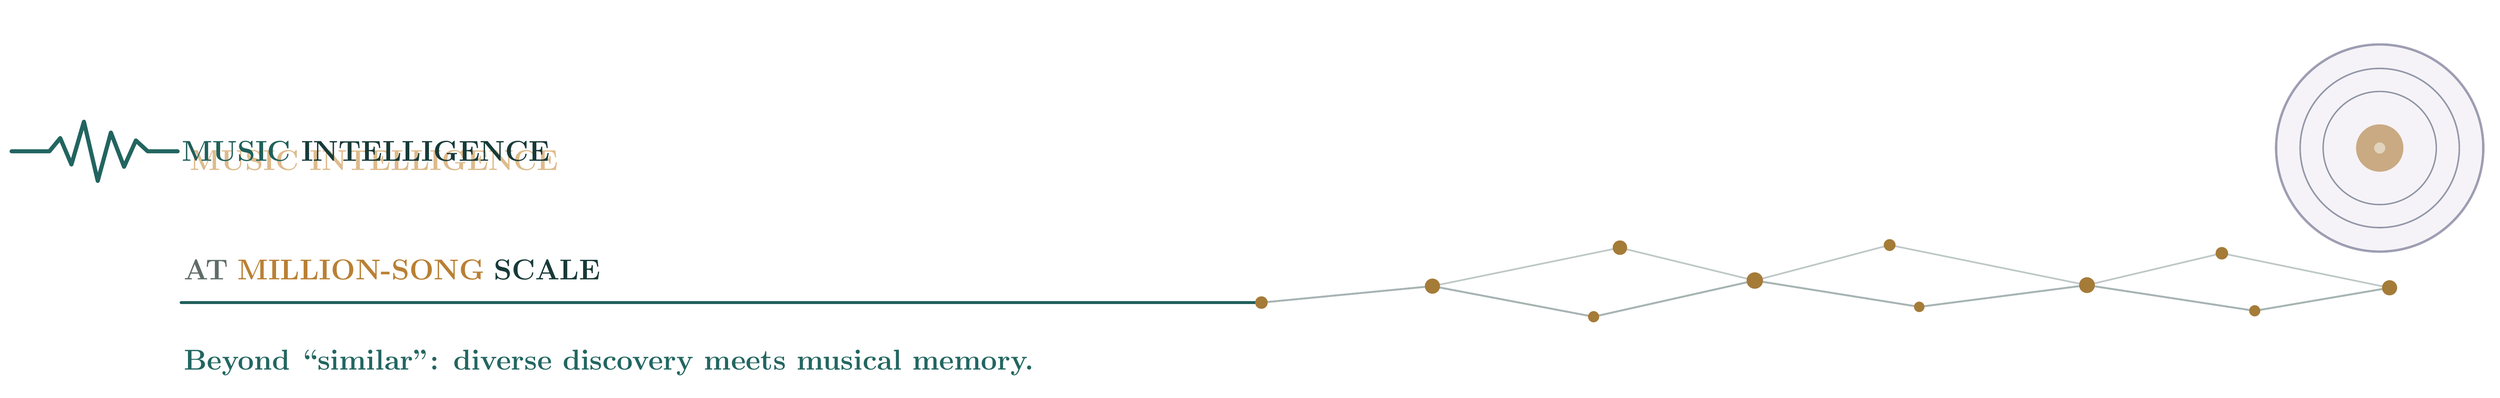
\begin{tikzpicture}[x=1cm,y=1cm,baseline=(current bounding box.north)]
    \path[use as bounding box] (0,0) rectangle (75.3,11.4);

    % A music waveform enters the wordmark from the left.
    \draw[posterteal!88!posterink,line width=1.25mm,line cap=round,line join=round]
      (0,7.15) -- (1.15,7.15) -- (1.48,7.55) -- (1.82,6.75)
      -- (2.20,8.05) -- (2.62,6.25) -- (3.02,7.72)
      -- (3.42,6.68) -- (3.78,7.48) -- (4.14,7.15) -- (5.05,7.15);

    % Warm offset print shadow, followed by the crisp foreground lettering.
    \node[anchor=west,font=\fontsize{104}{108}\selectfont\bfseries,
      text=postergold!52!posterpaper] at (5.30,6.88)
      {MUSIC INTELLIGENCE};
    \node[anchor=west,font=\fontsize{104}{108}\selectfont\bfseries]
      at (5.05,7.15)
      {{\color{posterteal!78!posterink}MUSIC}\hspace{.32cm}{\color{posterink}INTELLIGENCE}};

    \node[anchor=west,font=\fontsize{45}{50}\selectfont\bfseries]
      at (5.12,3.55)
      {{\color{postermuted}AT}\hspace{.28cm}{\color{postergold!92!black}MILLION-SONG}\hspace{.28cm}{\color{posterink}SCALE}};

    % The signal becomes a small data network under the scale line.
    \draw[posterteal!76!posterink,line width=.78mm,line cap=round]
      (5.15,2.55) -- (38.0,2.55);
    \draw[posterink!38,line width=.58mm]
      (38.0,2.55) -- (43.2,3.05) -- (48.1,2.12) -- (53.0,3.22)
      -- (58.0,2.42) -- (63.1,3.08) -- (68.2,2.30) -- (72.3,3.00);
    \draw[posterink!28,line width=.50mm]
      (43.2,3.05) -- (48.9,4.22) -- (53.0,3.22) -- (57.1,4.30)
      -- (63.1,3.08) -- (67.2,4.05) -- (72.3,3.00);
    \foreach \x/\y/\r in {
      38.0/2.55/.19,43.2/3.05/.23,48.1/2.12/.17,48.9/4.22/.22,
      53.0/3.22/.25,57.1/4.30/.18,58.0/2.42/.16,63.1/3.08/.24,
      67.2/4.05/.19,68.2/2.30/.17,72.3/3.00/.23}
      \fill[postergold!80!posterink] (\x,\y) circle (\r cm);

    % A subtle record anchors the nostalgic side of the identity.
    \begin{scope}[opacity=.58]
      \fill[posterpurple!13] (72.0,7.25) circle (3.15cm);
      \draw[posterpurple!72!posterink,line width=.72mm] (72.0,7.25) circle (3.15cm);
      \draw[posterpurple!58!posterink,line width=.46mm] (72.0,7.25) circle (2.42cm);
      \draw[posterpurple!48!posterink,line width=.42mm] (72.0,7.25) circle (1.72cm);
      \fill[postergold!85!black] (72.0,7.25) circle (.72cm);
      \fill[posterpaper] (72.0,7.25) circle (.17cm);
    \end{scope}

    \node[anchor=west,font=\fontsize{31}{37}\selectfont\bfseries,
      text=posterteal!90!posterink] at (5.12,.72)
      {Beyond ``similar'': diverse discovery meets musical memory.};
  \end{tikzpicture}
\end{textblock}

% Product story ----------------------------------------------------------------
% Disabled while the title artwork is being designed.
\newcommand{\disabledtargetpanel}{%
\begin{textblock}{58}(4,13.0)
  \begin{musicpanel}[height=16.2cm]{posterteal}
    \sectiontitle{Our target: one song, three experiences.}
    \vspace{.12cm}
    {\fontsize{28}{34}\selectfont\color{postermuted}
      Turn one query into catalog insight, diverse recommendations, and a journey through musical time.\par}
    \vspace{.08cm}
    \begin{center}
      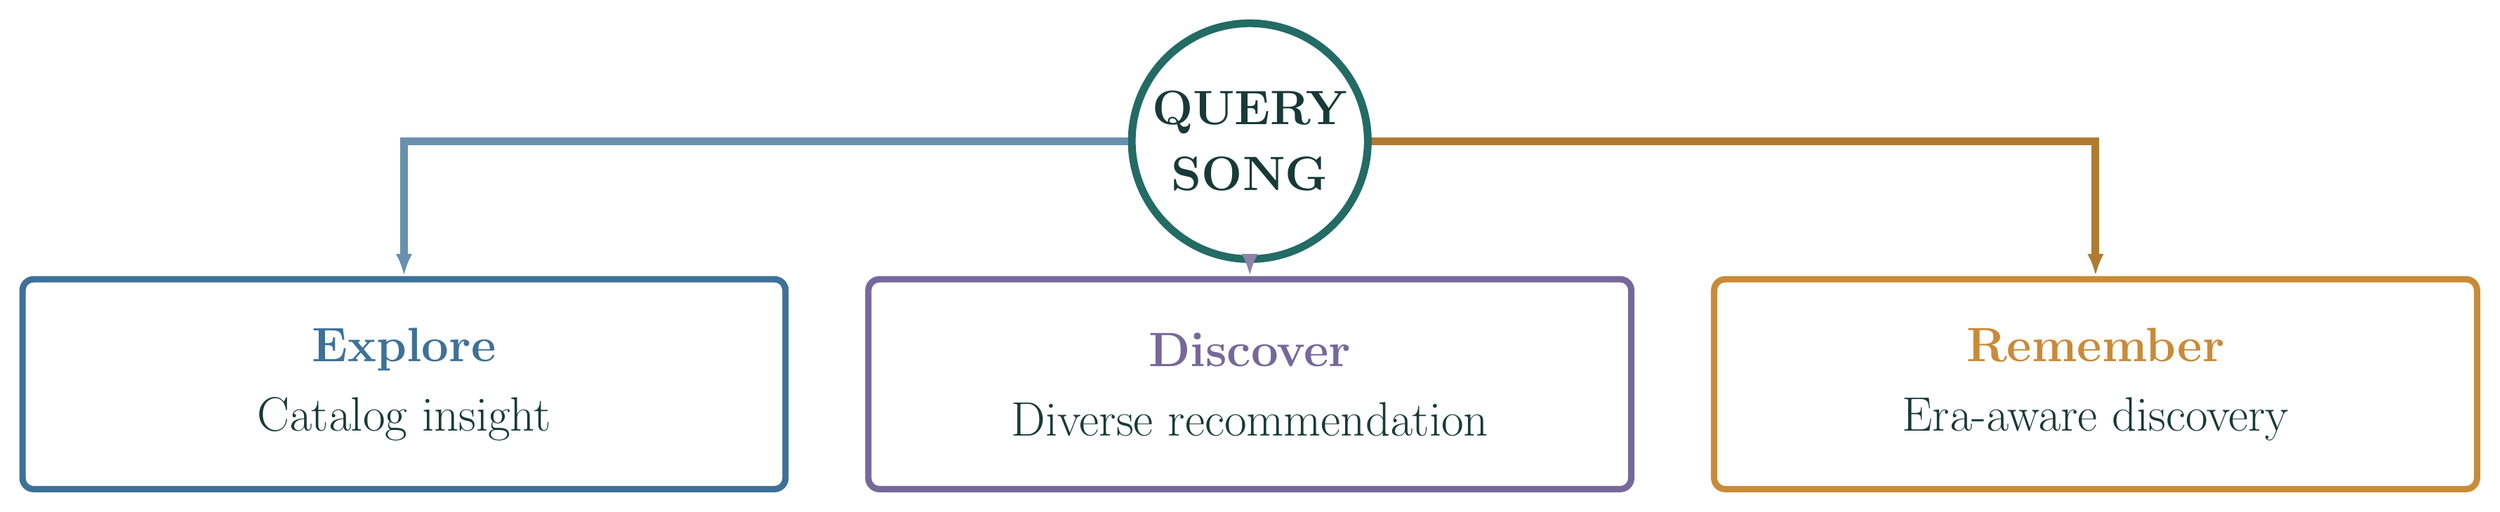
\begin{tikzpicture}[
        >=Latex,
        flow/.style={-{Latex[length=4mm,width=3mm]},line width=1.4mm},
        query/.style={circle,minimum size=3.65cm,line width=1.4mm,
          draw=posterteal,fill=white,fill opacity=.72,text opacity=1,
          font=\fontsize{30}{34}\selectfont\bfseries,align=center,text=posterink},
        outcome/.style={rounded corners=2mm,minimum width=13.8cm,minimum height=3.8cm,
          line width=1.15mm,align=center,fill=white,fill opacity=.68,text opacity=1,
          font=\fontsize{28}{33}\selectfont,text=posterink}
      ]
        \node[query] (song) at (0,2.35) {QUERY\\SONG};

        \node[outcome,draw=posterblue] (explore) at (-15.3,-2.05) {
          {\fontsize{34}{38}\selectfont\bfseries\color{posterblue}Explore}\\[.10cm]
          Catalog insight};
        \node[outcome,draw=posterpurple] (discover) at (0,-2.05) {
          {\fontsize{34}{38}\selectfont\bfseries\color{posterpurple}Discover}\\[.10cm]
          Diverse recommendation};
        \node[outcome,draw=postergold] (remember) at (15.3,-2.05) {
          {\fontsize{34}{38}\selectfont\bfseries\color{postergold}Remember}\\[.10cm]
          Era-aware discovery};

        \draw[flow,draw=posterblue!78] (song.west) -| (explore.north);
        \draw[flow,draw=posterpurple!82] (song.south) -- (discover.north);
        \draw[flow,draw=postergold!88!black] (song.east) -| (remember.north);
      \end{tikzpicture}
    \end{center}
    \vspace{-.20cm}
    \begin{center}
      {\fontsize{27}{32}\selectfont\bfseries\color{posterink}
        Big-data method: 267 GB HDF5 $\rightarrow$ Avro/Parquet $\rightarrow$ Drill + Spark $\rightarrow$ FAISS + learned models}
    \end{center}
  \end{musicpanel}
\end{textblock}
}

% Better discovery -------------------------------------------------------------
% Disabled while the five-panel visual system is being designed.
\newcommand{\disabledevidencepanels}{%
\begin{textblock}{29.5}(4,59.2)
  \begin{musicpanel}[height=19.0cm]{posterpurple}
    \sectiontitle{Better discovery}
    \smallnote{Relation-aware vs. release-only retrieval}
    \vspace{.65cm}

    \begin{center}
      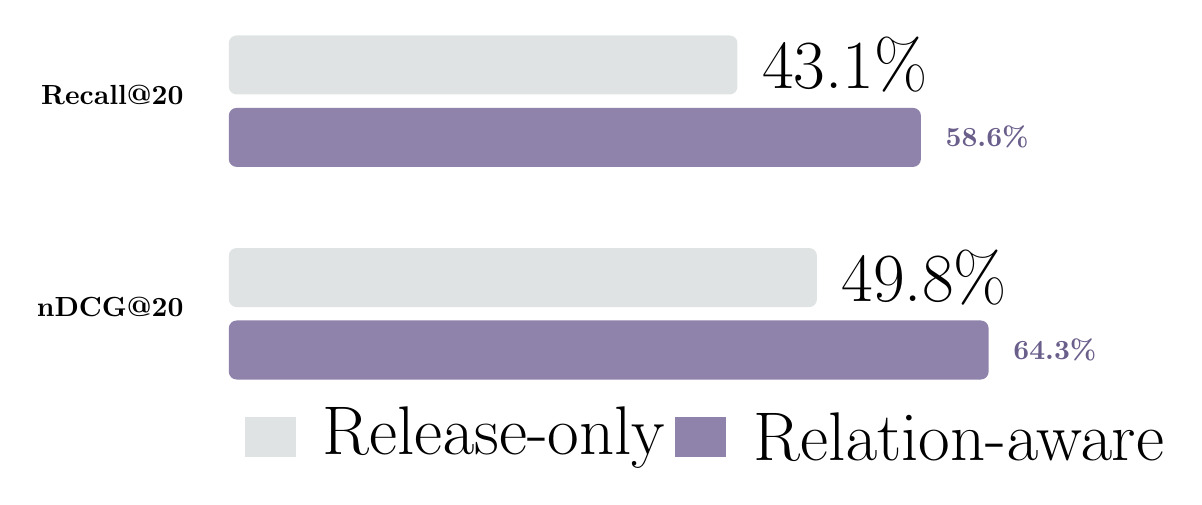
\begin{tikzpicture}[x=1cm,y=1cm,font=\fontsize{23}{27}\selectfont]
        \node[anchor=east,font=\bfseries] at (0,3.60) {Recall@20};
        \node[anchor=east,font=\bfseries] at (0,.90) {nDCG@20};

        \fill[posterink!14,rounded corners=1mm] (.45,3.60) rectangle (6.91,4.35);
        \fill[posterpurple!82,rounded corners=1mm] (.45,2.68) rectangle (9.24,3.43);
        \fill[posterink!14,rounded corners=1mm] (.45,.90) rectangle (7.92,1.65);
        \fill[posterpurple!82,rounded corners=1mm] (.45,-.02) rectangle (10.10,.73);

        \node[anchor=west] at (7.10,3.98) {43.1\%};
        \node[anchor=west,font=\bfseries,text=posterpurple!90!black] at (9.43,3.06) {58.6\%};
        \node[anchor=west] at (8.11,1.28) {49.8\%};
        \node[anchor=west,font=\bfseries,text=posterpurple!90!black] at (10.29,.36) {64.3\%};

        \fill[posterink!14] (.65,-1.00) rectangle (1.30,-.50);
        \node[anchor=west] at (1.52,-.75) {Release-only};
        \fill[posterpurple!82] (6.12,-1.00) rectangle (6.77,-.50);
        \node[anchor=west] at (6.99,-.75) {Relation-aware};
      \end{tikzpicture}
    \end{center}

    \vspace{.65cm}
    \begin{center}
      {\fontsize{58}{62}\selectfont\bfseries\color{posterpurple}+15.6 pp\par}
      {\fontsize{31}{36}\selectfont\bfseries Recall@20\par}
      \vspace{.35cm}
      {\fontsize{31}{36}\selectfont\bfseries\color{posterink}+14.5 pp nDCG@20\par}
    \end{center}

    \vfill
    \begin{center}
      {\fontsize{25}{30}\selectfont\color{postermuted}10,000-query offline benchmark}
    \end{center}
  \end{musicpanel}
\end{textblock}

% Faster graph intelligence ----------------------------------------------------
\begin{textblock}{29.5}(35.25,42.8)
  \begin{musicpanel}[height=19.0cm]{posterblue}
    \sectiontitle{Faster graph intelligence}
    \smallnote{Same graph. Same verified answer.}
    \vspace{.65cm}

    \begin{center}
      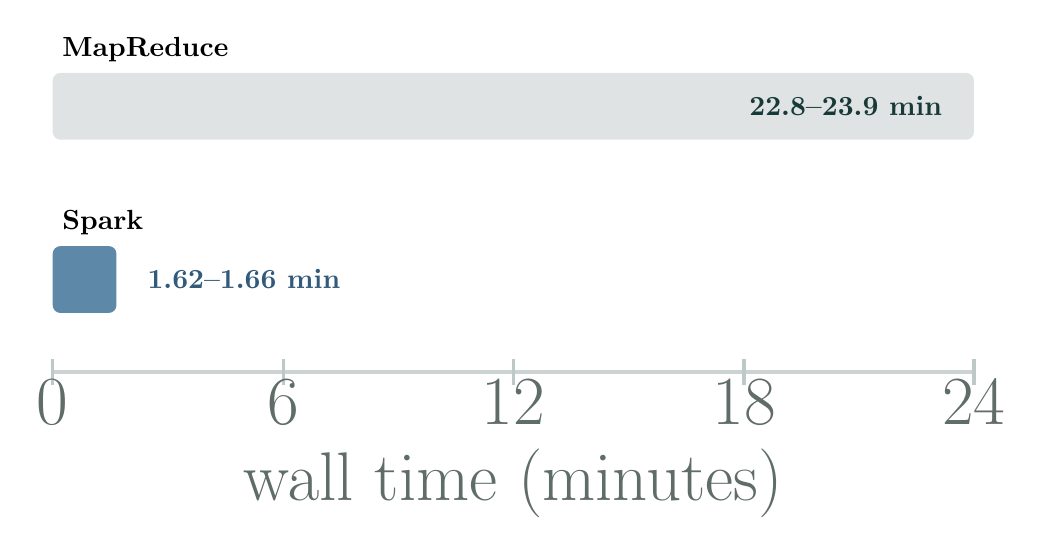
\begin{tikzpicture}[x=1cm,y=1cm,font=\fontsize{24}{28}\selectfont]
        \node[anchor=west,font=\bfseries] at (0,4.45) {MapReduce};
        \fill[posterink!14,rounded corners=1mm] (0,3.30) rectangle (11.7,4.15);
        \node[anchor=east,font=\bfseries,text=posterink] at (11.42,3.73) {22.8--23.9 min};

        \node[anchor=west,font=\bfseries] at (0,2.25) {Spark};
        \fill[posterblue!84,rounded corners=1mm] (0,1.10) rectangle (.81,1.95);
        \node[anchor=west,font=\bfseries,text=posterblue!80!black] at (1.08,1.53) {1.62--1.66 min};

        \draw[line width=.55mm,draw=posterink!22] (0,.35) -- (11.7,.35);
        \foreach \x/\lab in {0/0,2.93/6,5.85/12,8.78/18,11.7/24}
          \draw[draw=posterink!28,line width=.4mm] (\x,.18) -- (\x,.52)
            node[below=.14cm,text=postermuted] {\lab};
        \node[below=.85cm,text=postermuted] at (5.85,.35) {wall time (minutes)};
      \end{tikzpicture}
    \end{center}

    \vspace{.70cm}
    \begin{center}
      {\fontsize{58}{62}\selectfont\bfseries\color{posterblue}14.1--14.4$\times$\par}
      {\fontsize{31}{36}\selectfont\bfseries faster with Spark\par}
    \end{center}

    \vfill
    \begin{center}
      {\fontsize{25}{30}\selectfont\color{postermuted}Five runs per combination . all outputs verified}
    \end{center}
  \end{musicpanel}
\end{textblock}

% Sharper era estimation -------------------------------------------------------
\begin{textblock}{29.5}(66.5,26.4)
  \begin{musicpanel}[height=19.0cm]{postergold}
    \sectiontitle{Sharper era estimation}
    \smallnote{Progressive improvement on held-out artists}
    \vspace{.55cm}

    \begin{center}
      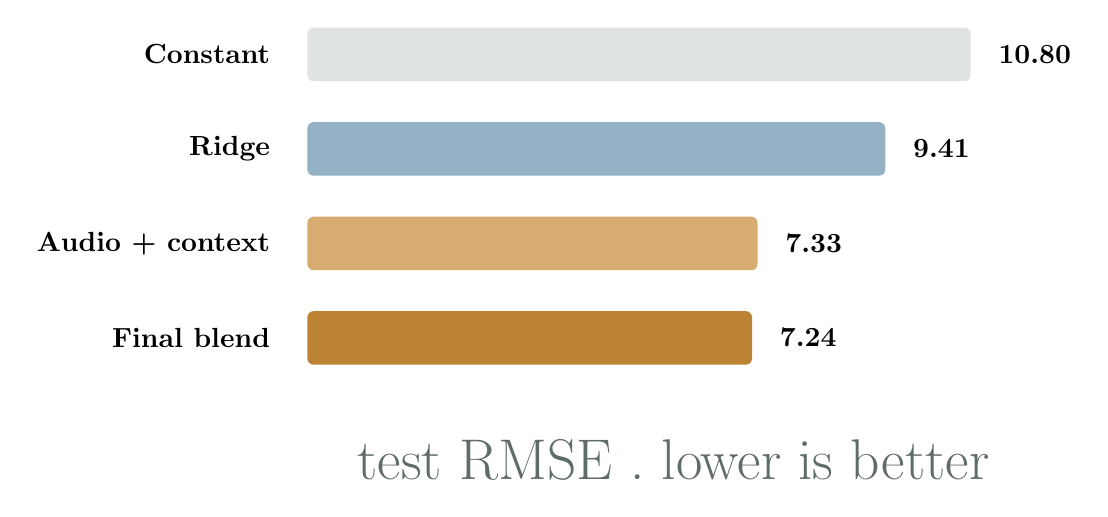
\begin{tikzpicture}[x=1cm,y=1cm,font=\fontsize{21}{25}\selectfont]
        \yearbar{3.65}{Constant}{10.80}{posterink!14}
        \yearbar{2.45}{Ridge}{9.41}{posterblue!55}
        \yearbar{1.25}{Audio + context}{7.33}{postergold!72}
        \yearbar{.05}{Final blend}{7.24}{postergold!94!black}
        \node[anchor=north,text=postermuted] at (5.0,-.78) {test RMSE . lower is better};
      \end{tikzpicture}
    \end{center}

    \vspace{.60cm}
    \begin{center}
      {\fontsize{58}{62}\selectfont\bfseries\color{postergold}7.24 years\par}
      {\fontsize{31}{36}\selectfont\bfseries final test RMSE\par}
      \vspace{.35cm}
      {\fontsize{31}{36}\selectfont\bfseries\color{posterink}23.0\% lower than Ridge\par}
      \vspace{.28cm}
      {\fontsize{27}{32}\selectfont\color{postermuted}Final MAE: 4.82 years\par}
    \end{center}

  \end{musicpanel}
\end{textblock}
}

% Investment close -------------------------------------------------------------
% Disabled while the title artwork is being designed.
\newcommand{\disabledinvestmentpanel}{%
\begin{textblock}{38}(58,76.6)
  \begin{musicpanel}[height=9.6cm]{posterteal}
    \sectiontitle{Why invest now?}
    \vspace{.52cm}
    {\fontsize{31}{36}\selectfont\bfseries\color{posterpurple}Differentiated}\quad
    {\fontsize{27}{32}\selectfont Discovery beyond nearest-neighbor lists.\par}
    \vspace{.42cm}
    {\fontsize{31}{36}\selectfont\bfseries\color{posterblue}Measured}\quad
    {\fontsize{27}{32}\selectfont One million tracks, reproducible evidence.\par}
    \vspace{.42cm}
    {\fontsize{31}{36}\selectfont\bfseries\color{postergold}Ready to learn}\quad
    {\fontsize{27}{32}\selectfont Online listener feedback is next.\par}
  \end{musicpanel}
\end{textblock}
}

% Five-panel visual skeleton ---------------------------------------------------
\begin{textblock}{29.5}(4,24.8)
  \begin{targetcard}[height=22.3cm]
    \resizebox{\linewidth}{!}{\targetmark}
    \vspace{-1.55cm}
    \begin{center}
      {\fontsize{38}{43}\selectfont\bfseries
        One query song.\\Three differentiated experiences.\par}
    \end{center}
    \vspace{-.02cm}
    \begin{center}
      \resizebox{.92\linewidth}{!}{%
      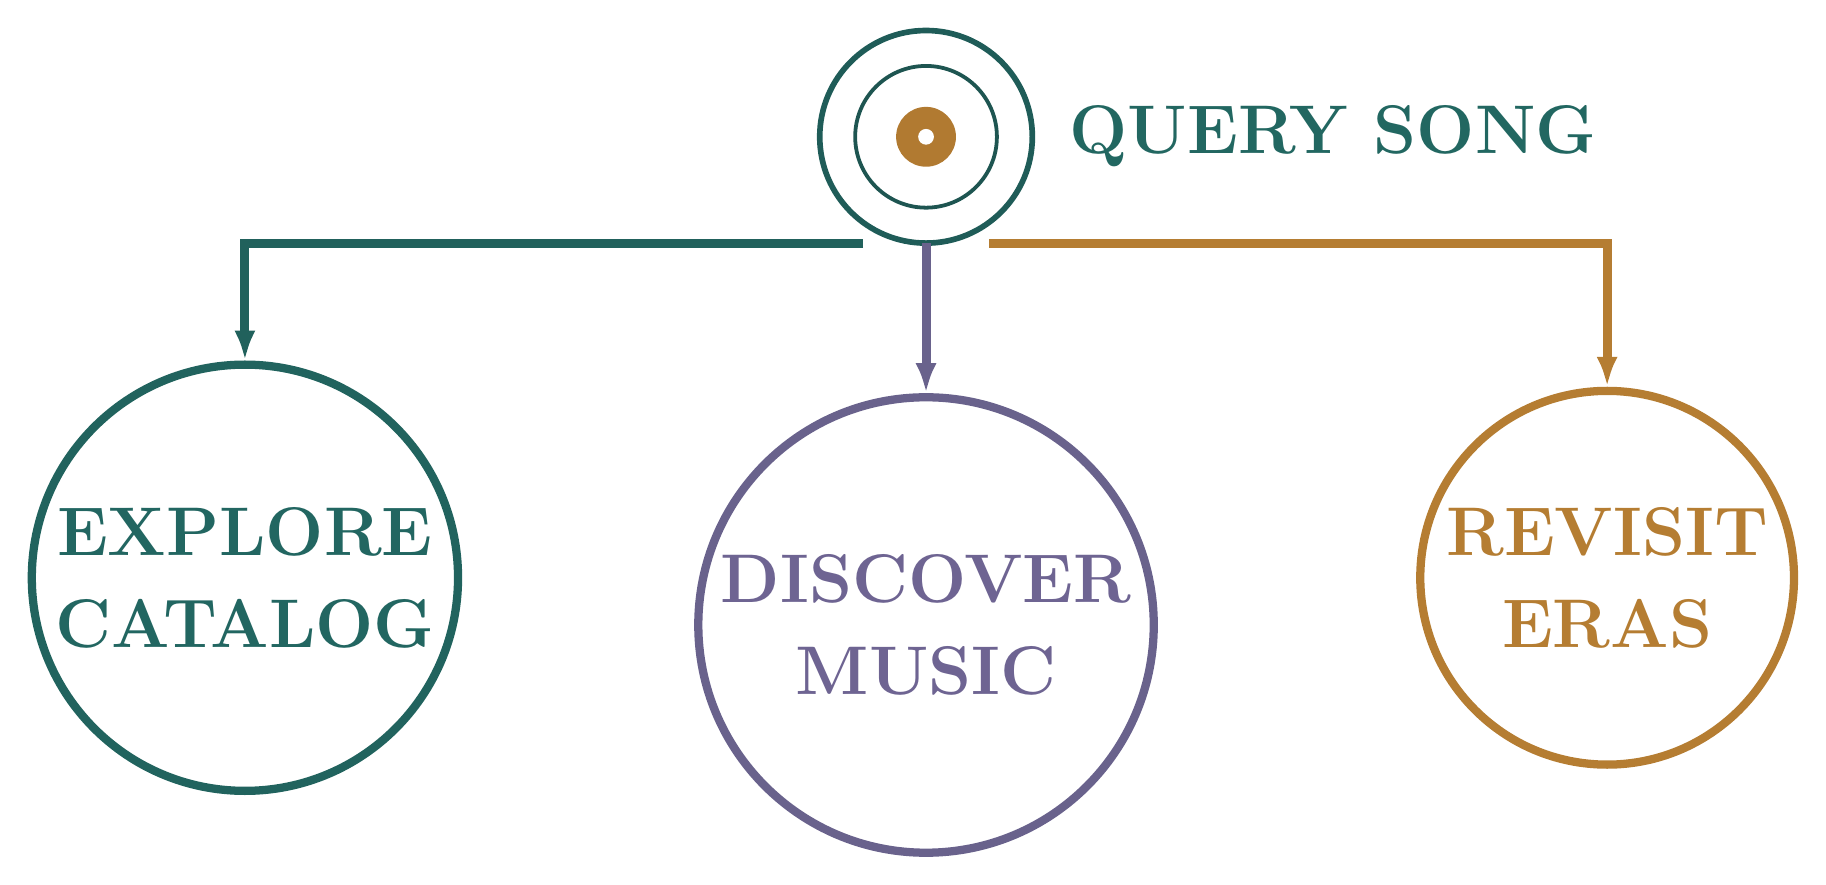
\begin{tikzpicture}[
        x=1cm,y=1cm,>=Latex,
        flow/.style={-{Latex[length=3.8mm,width=2.7mm]},line width=1.15mm},
        outcome/.style={circle,minimum size=3.65cm,line width=1.05mm,
          fill=white,fill opacity=.50,text opacity=1,align=center,
          font=\fontsize{30}{33}\selectfont\bfseries}
      ]
        \draw[posterteal!70!posterink,line width=.72mm] (12.35,7.35) circle (1.35cm);
        \draw[posterteal!55!posterink,line width=.48mm] (12.35,7.35) circle (.90cm);
        \fill[postergold!88!black] (12.35,7.35) circle (.38cm);
        \fill[white] (12.35,7.35) circle (.10cm);
        \node[anchor=west,font=\fontsize{25}{28}\selectfont\bfseries,
          text=posterteal!92!posterink] at (14.05,7.35) {QUERY SONG};

        \node[outcome,draw=posterteal!84!posterink,text=posterteal!90!posterink]
          (catalog) at (3.7,1.75) {EXPLORE\\CATALOG};
        \node[outcome,draw=posterpurple!86!posterink,text=posterpurple!92!posterink]
          (discover) at (12.35,1.15) {DISCOVER\\MUSIC};
        \node[outcome,draw=postergold!90!black,text=postergold!90!black]
          (remember) at (21.0,1.75) {REVISIT\\ERAS};

        \draw[flow,draw=posterteal!80!posterink]
          (11.55,6.00) -| (catalog.north);
        \draw[flow,draw=posterpurple!86!posterink]
          (12.35,6.00) -- (discover.north);
        \draw[flow,draw=postergold!90!black]
          (13.15,6.00) -| (remember.north);
      \end{tikzpicture}%
      }
    \end{center}
    \vspace{.12cm}
    \begin{center}
      {\fontsize{26}{30}\selectfont\bfseries\color{postermuted}ONE REUSABLE DATA FOUNDATION\par}
      \vspace{.18cm}
      \resizebox{.92\linewidth}{!}{%
      
\begin{tikzpicture}[
        x=1cm,y=1cm,>=Latex,
        data/.style={align=center,font=\fontsize{28}{31}\selectfont\bfseries},
        pipe/.style={-{Latex[length=3mm,width=2.2mm]},draw=posterteal!82!posterink,
          line width=.92mm}
      ]
        \node[data,text=posterink] (raw) at (2.5,0) {267 GB\\HDF5};
        \node[data,text=posterpurple!92!posterink] (lake) at (9.1,0) {1M TRACKS\\PARQUET};
        \node[data,text=posterink] (engines) at (18.8,0) {DRILL \textbullet\ SPARK\\FAISS \textbullet\ MODELS};
        \draw[pipe] (raw.east) -- (lake.west);
        \draw[pipe] (lake.east) -- (engines.west);
      \end{tikzpicture}%
      }
    \end{center}
  \end{targetcard}
\end{textblock}

\begin{textblock}{29.5}(35.25,24.8)
  \begin{discoverycard}[height=22.3cm]
    \resizebox{\linewidth}{!}{\discoverymark}
    \vspace{-.95cm}
    \begin{center}
      \resizebox{.94\linewidth}{!}{%
      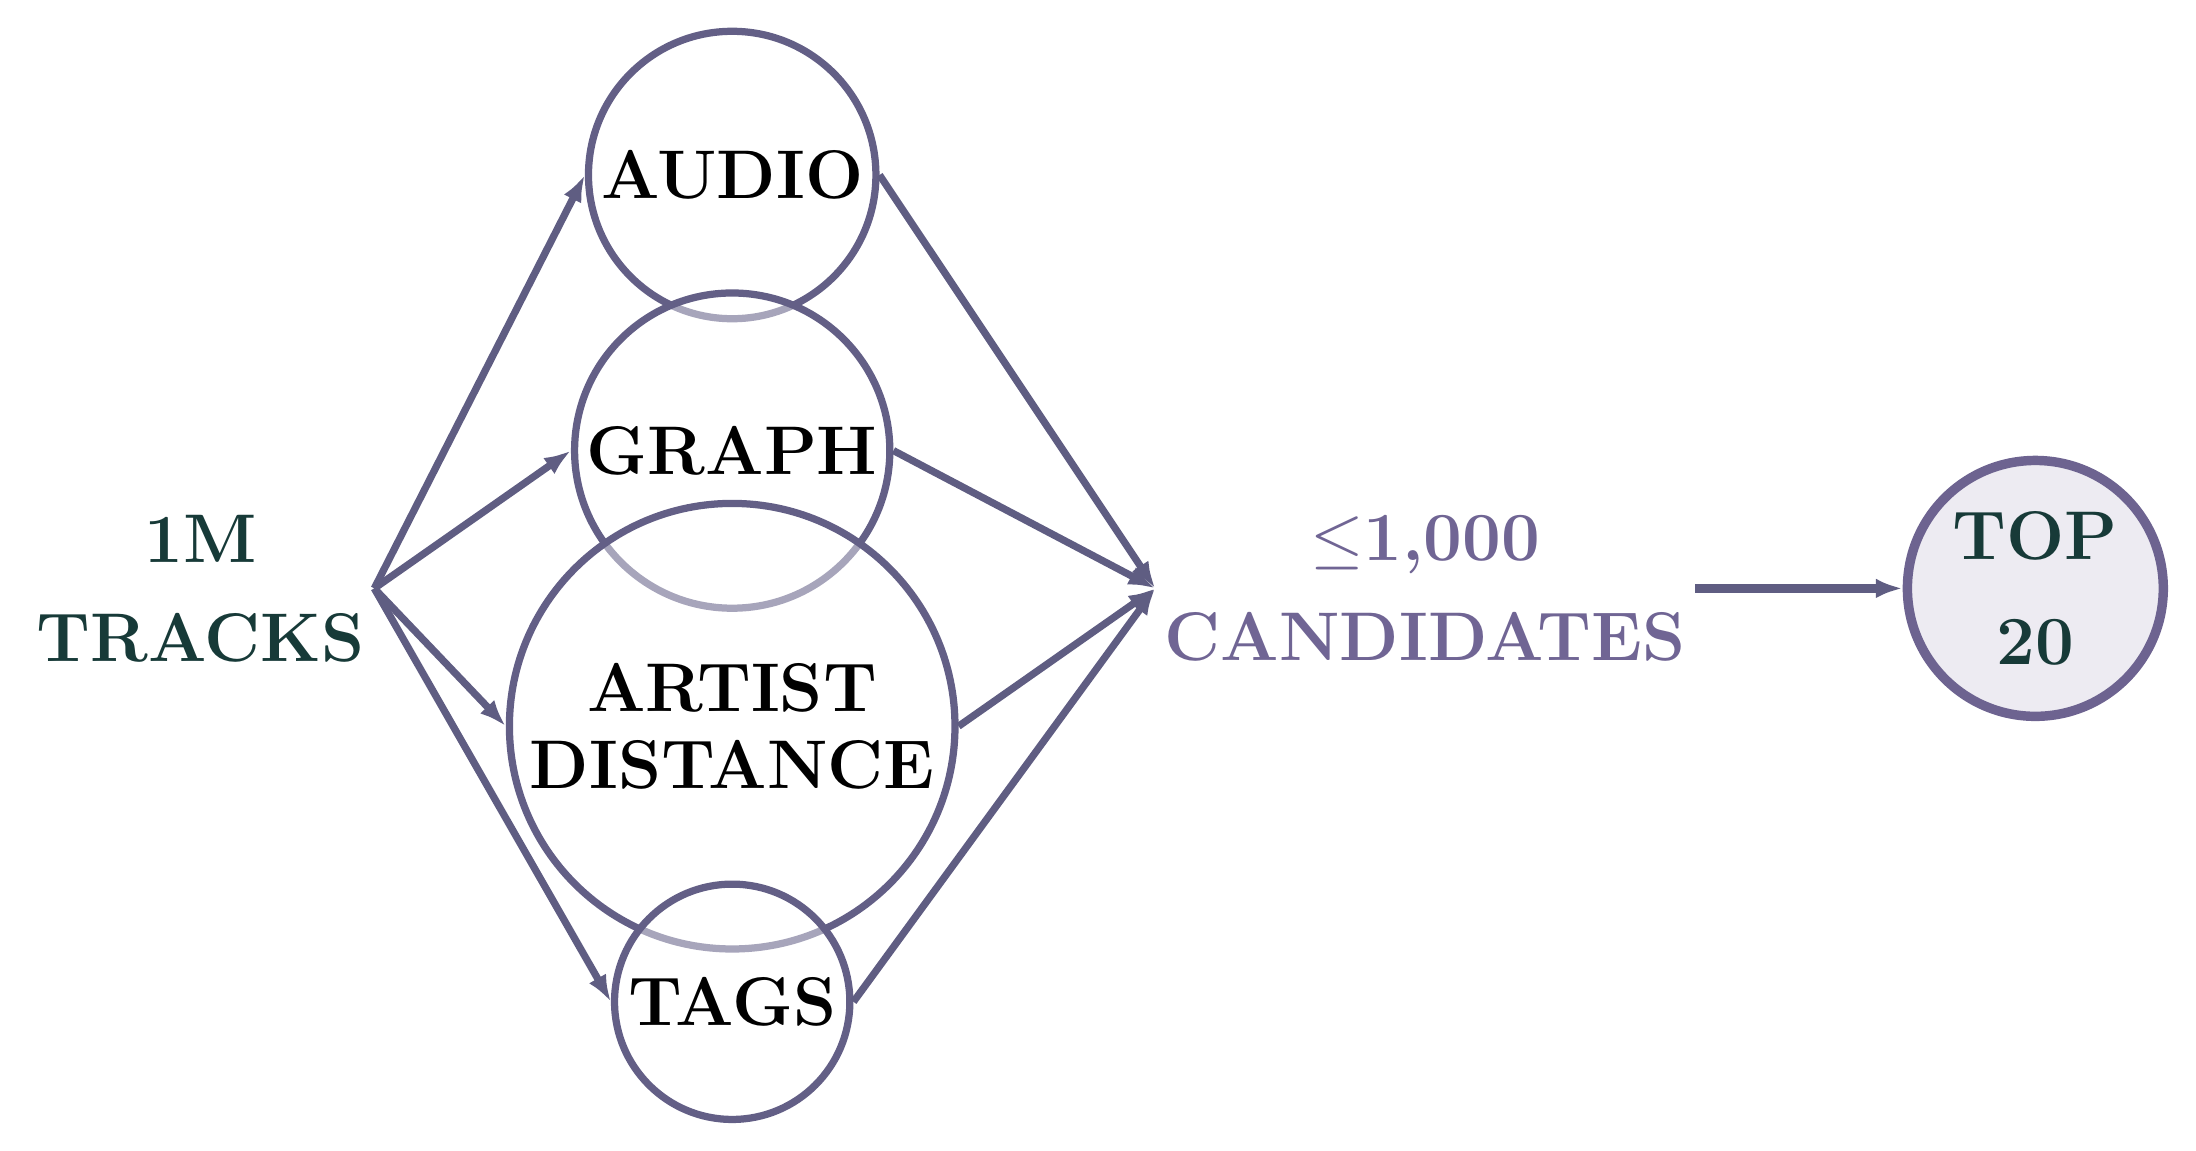
\begin{tikzpicture}[
        x=1cm,y=1cm,>=Latex,
        source/.style={circle,minimum size=2.85cm,line width=.92mm,
          draw=posterpurple!80!posterink,fill=white,fill opacity=.44,text opacity=1,
          align=center,font=\fontsize{25}{28}\selectfont\bfseries},
        flow/.style={-{Latex[length=3.4mm,width=2.5mm]},draw=posterpurple!76!posterink,
          line width=.92mm}
      ]
        \node[align=center,font=\fontsize{32}{36}\selectfont\bfseries,text=posterink]
          (catalog) at (.45,5.35) {1M\\TRACKS};

        \node[source] (audio) at (7.2,10.60) {AUDIO};
        \node[source] (graph) at (7.2,7.10) {GRAPH};
        \node[source] (bfs) at (7.2,3.60) {ARTIST\\DISTANCE};
        \node[source] (tags) at (7.2,.10) {TAGS};

        \node[align=center,font=\fontsize{32}{36}\selectfont\bfseries,
          text=posterpurple!94!posterink] (shortlist) at (16.0,5.35)
          {$\leq$1,000\\CANDIDATES};
        \node[circle,minimum size=3.25cm,line width=1.2mm,
          draw=posterpurple!90!posterink,fill=posterpurple!13,
          align=center,font=\fontsize{34}{38}\selectfont\bfseries,text=posterink]
          (topk) at (23.75,5.35) {TOP\\20};

        \foreach \s in {audio,graph,bfs,tags}{
          \draw[flow] (catalog.east) -- (\s.west);
          \draw[flow] (\s.east) -- (shortlist.west);
        }
        \draw[flow,line width=1.18mm] (shortlist.east) -- (topk.west);
      \end{tikzpicture}%
      }
    \end{center}
    \vspace{-.40cm}
    \begin{center}
      \resizebox{.94\linewidth}{!}{%
      
\begin{tikzpicture}[x=1cm,y=1cm]
        \draw[posterpurple!35,line width=.5mm] (8.15,-.20) -- (8.15,2.05);
        \draw[posterpurple!35,line width=.5mm] (16.35,-.20) -- (16.35,2.05);
        \node[align=center,font=\fontsize{41}{45}\selectfont\bfseries,
          text=posterpurple!94!posterink] at (4.0,1.08) {128D\\AUDIO};
        \node[align=center,font=\fontsize{41}{45}\selectfont\bfseries,
          text=posterpurple!94!posterink] at (12.25,1.08) {10M\\WALKS};
        \node[align=center,font=\fontsize{41}{45}\selectfont\bfseries,
          text=posterpurple!94!posterink] at (20.5,1.08) {400M\\TOKENS};
      \end{tikzpicture}%
      }
      \vspace{.58cm}
      {\fontsize{29}{33}\selectfont\bfseries\color{postermuted}
        SPARK ML \textbullet\ WORD2VEC \textbullet\ FAISS\par}
    \end{center}
  \end{discoverycard}
\end{textblock}

\begin{textblock}{29.5}(66.5,24.8)
  \begin{graphcard}[height=22.3cm]
    \resizebox{\linewidth}{!}{\graphmark}
    \vspace{-.48cm}
    \begin{center}
      {\fontsize{77}{80}\selectfont\bfseries\color{posterpurple!95!posterink}14.4$\times$\par}
      \vspace{-.08cm}
      {\fontsize{36}{40}\selectfont\bfseries Spark acceleration\par}
    \end{center}
    \vspace{.28cm}
    \begin{center}
      \resizebox{.97\linewidth}{!}{%
      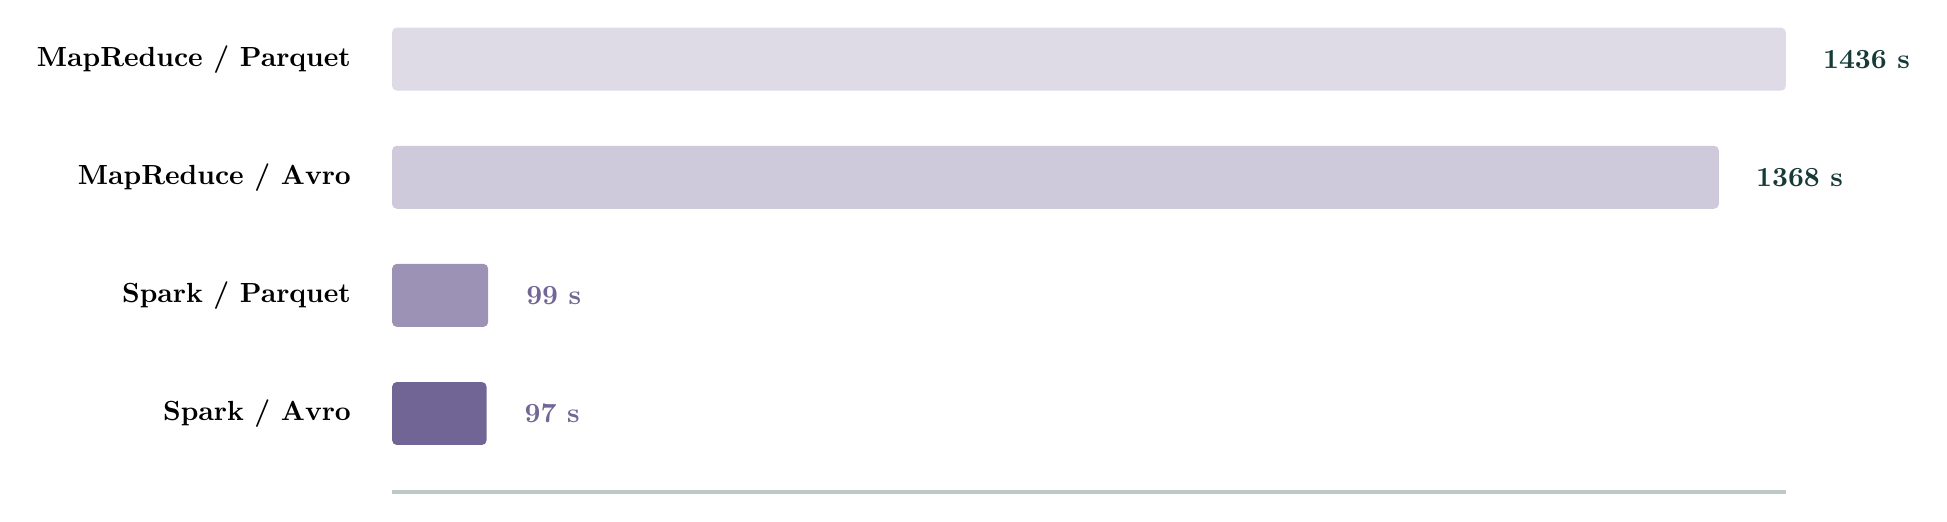
\begin{tikzpicture}[x=1cm,y=1cm,font=\fontsize{28}{31}\selectfont]
        \node[anchor=east,font=\bfseries] at (5.1,5.75) {MapReduce / Parquet};
        \fill[posterpurple!24,rounded corners=.6mm] (5.5,5.35) rectangle (23.2,6.15);
        \node[anchor=west,font=\bfseries,text=posterink] at (23.55,5.75) {1436 s};

        \node[anchor=east,font=\bfseries] at (5.1,4.25) {MapReduce / Avro};
        \fill[posterpurple!36,rounded corners=.6mm] (5.5,3.85) rectangle (22.35,4.65);
        \node[anchor=west,font=\bfseries,text=posterink] at (22.70,4.25) {1368 s};

        \node[anchor=east,font=\bfseries] at (5.1,2.75) {Spark / Parquet};
        \fill[posterpurple!72,rounded corners=.6mm] (5.5,2.35) rectangle (6.72,3.15);
        \node[anchor=west,font=\bfseries,text=posterpurple!95!posterink] at (7.08,2.75) {99 s};

        \node[anchor=east,font=\bfseries] at (5.1,1.25) {Spark / Avro};
        \fill[posterpurple!94!posterink,rounded corners=.6mm] (5.5,.85) rectangle (6.70,1.65);
        \node[anchor=west,font=\bfseries,text=posterpurple!95!posterink] at (7.06,1.25) {97 s};

        \draw[posterink!28,line width=.48mm] (5.5,.25) -- (23.2,.25);
      \end{tikzpicture}%
      }
    \end{center}
    \vfill
    \begin{center}
      {\fontsize{31}{35}\selectfont\bfseries\color{posterink}
        5 RUNS $\times$ 4 COMBINATIONS\par}
      \vspace{.12cm}
      {\fontsize{32}{36}\selectfont\bfseries\color{postermuted}
        Spark / MapReduce \textbullet\ Avro / Parquet\par}
    \end{center}
  \end{graphcard}
\end{textblock}

\begin{textblock}{29.5}(4,66.2)
  \begin{investmentcard}[height=17cm]
    \resizebox{\linewidth}{!}{\investmentmark}
    \vspace{-.85cm}
    \begin{center}
      \resizebox{.94\linewidth}{!}{%
      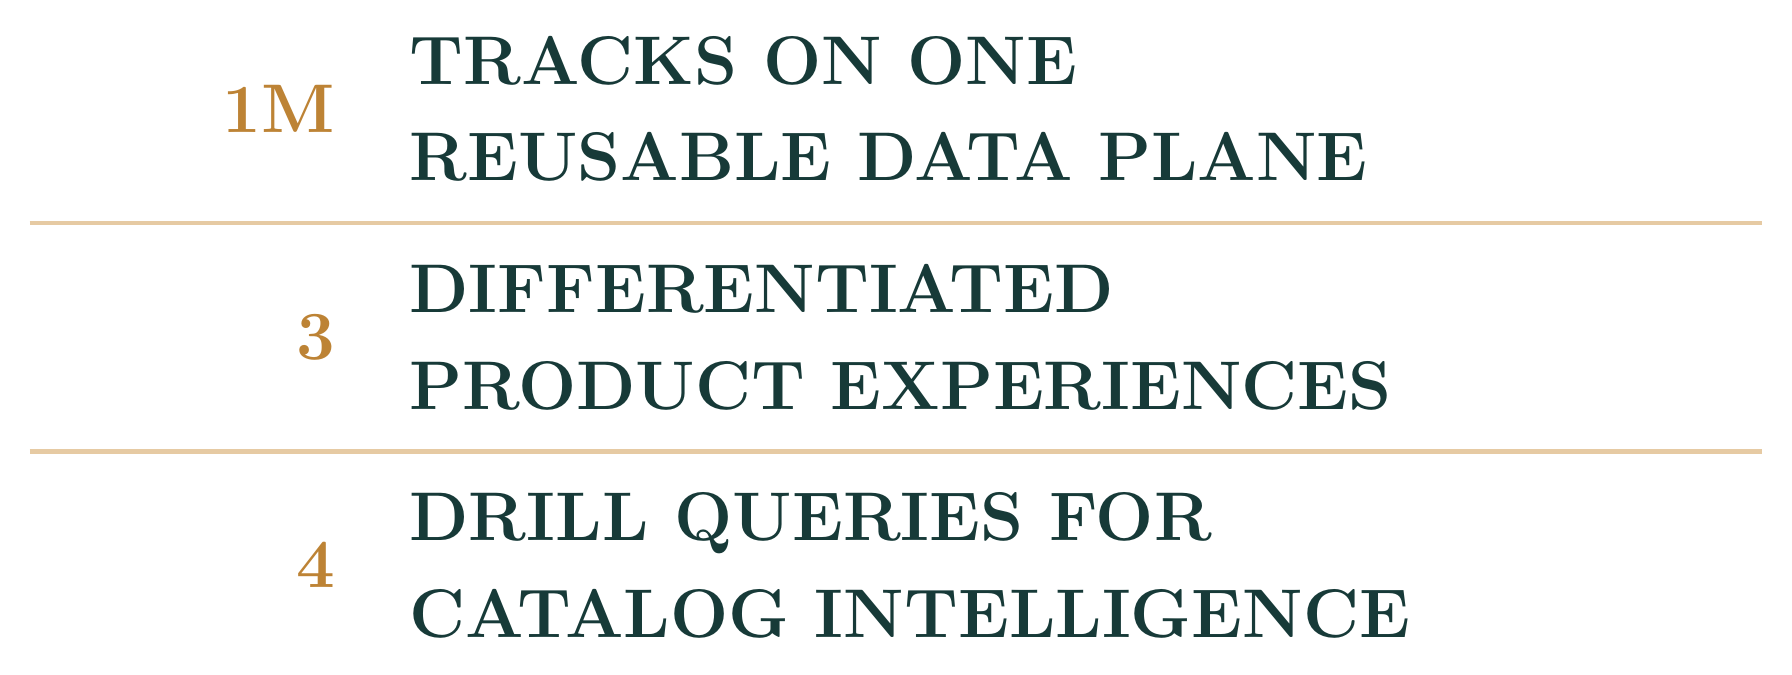
\begin{tikzpicture}[x=1cm,y=1cm]
        \node[anchor=east,font=\fontsize{57}{61}\selectfont\bfseries,
          text=postergold!94!black] at (5.0,6.45) {1M};
        \node[anchor=west,align=left,font=\fontsize{31}{35}\selectfont\bfseries,
          text=posterink] at (5.7,6.45) {TRACKS ON ONE\\REUSABLE DATA PLANE};

        \node[anchor=east,font=\fontsize{57}{61}\selectfont\bfseries,
          text=postergold!94!black] at (5.0,3.55) {3};
        \node[anchor=west,align=left,font=\fontsize{31}{35}\selectfont\bfseries,
          text=posterink] at (5.7,3.55) {DIFFERENTIATED\\PRODUCT EXPERIENCES};

        \node[anchor=east,font=\fontsize{57}{61}\selectfont\bfseries,
          text=postergold!94!black] at (5.0,.65) {4};
        \node[anchor=west,align=left,font=\fontsize{31}{35}\selectfont\bfseries,
          text=posterink] at (5.7,.65) {DRILL QUERIES FOR\\CATALOG INTELLIGENCE};

        \draw[postergold!46,line width=.52mm] (1.0,5.00) -- (23.0,5.00);
        \draw[postergold!46,line width=.52mm] (1.0,2.10) -- (23.0,2.10);
      \end{tikzpicture}%
      }
    \end{center}
    \vspace{.18cm}
    \begin{center}
      {\fontsize{27}{31}\selectfont\bfseries\color{postermuted}
        HADOOP \textbullet\ PARQUET \textbullet\ DRILL\\
        SPARK \textbullet\ FAISS\par}
    \end{center}
  \end{investmentcard}
\end{textblock}

\begin{textblock}{60.75}(35.25,66.2)
  \begin{eracard}[height=17cm]
    \resizebox{\linewidth}{!}{\eramark}
    \vspace{-.48cm}
    \begin{center}
      \resizebox{.96\linewidth}{!}{%
      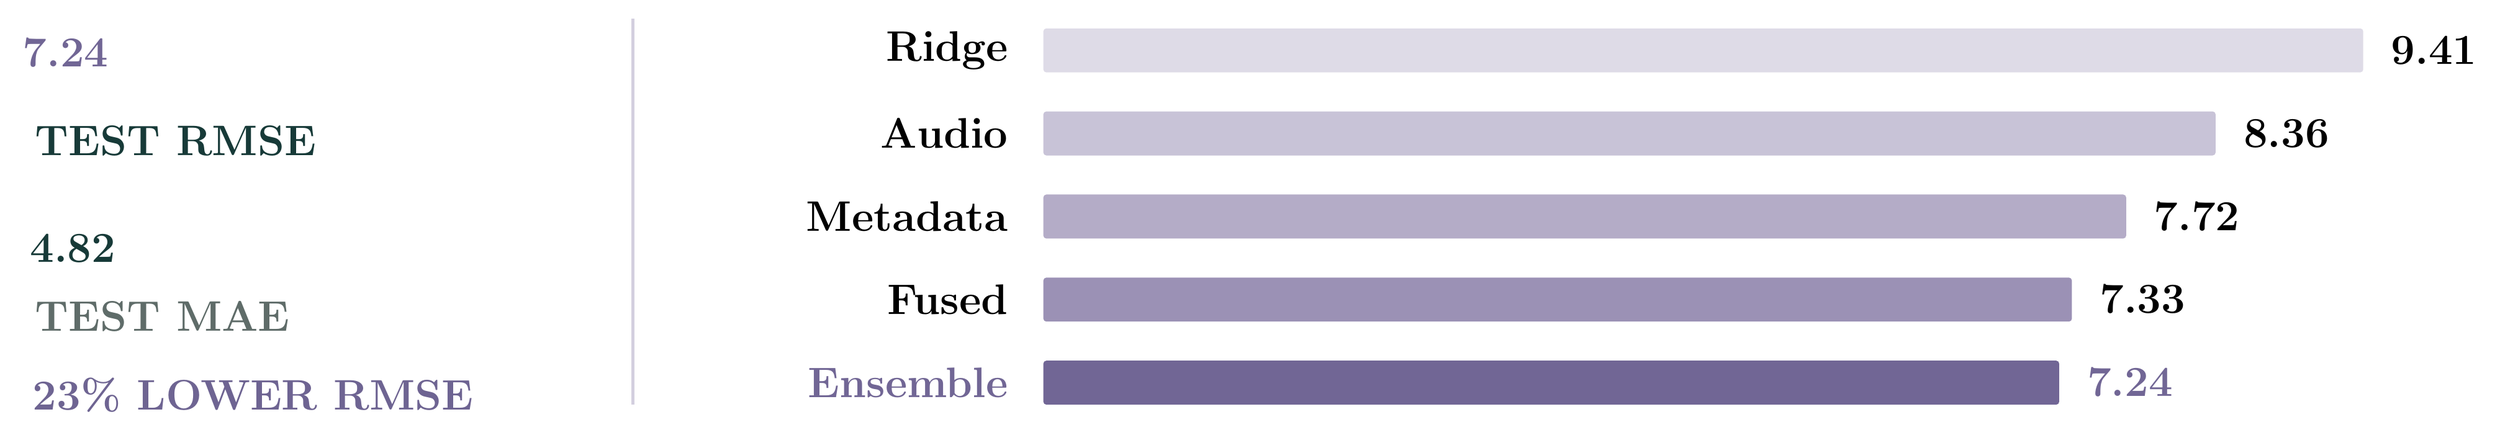
\begin{tikzpicture}[x=1cm,y=1cm]
        \node[anchor=west,font=\fontsize{82}{85}\selectfont\bfseries,
          text=posterpurple!95!posterink] at (0,7.05) {7.24};
        \node[anchor=west,font=\fontsize{33}{37}\selectfont\bfseries,
          text=posterink] at (.25,5.25) {TEST RMSE};
        \node[anchor=west,font=\fontsize{52}{56}\selectfont\bfseries,
          text=posterink] at (.15,3.05) {4.82};
        \node[anchor=west,font=\fontsize{31}{35}\selectfont\bfseries,
          text=postermuted] at (.25,1.65) {TEST MAE};
        \node[anchor=west,font=\fontsize{32}{36}\selectfont\bfseries,
          text=posterpurple!92!posterink] at (.20,.05) {23\% LOWER RMSE};

        \draw[posterpurple!32,line width=.60mm] (12.6,-.15) -- (12.6,7.75);

        \node[anchor=east,font=\fontsize{28}{31}\selectfont\bfseries] at (20.4,7.10) {Ridge};
        \fill[posterpurple!24,rounded corners=.6mm] (21.0,6.65) rectangle (48.0,7.55);
        \node[anchor=west,font=\fontsize{28}{31}\selectfont\bfseries] at (48.45,7.10) {9.41};

        \node[anchor=east,font=\fontsize{28}{31}\selectfont\bfseries] at (20.4,5.40) {Audio};
        \fill[posterpurple!40,rounded corners=.6mm] (21.0,4.95) rectangle (44.98,5.85);
        \node[anchor=west,font=\fontsize{28}{31}\selectfont\bfseries] at (45.43,5.40) {8.36};

        \node[anchor=east,font=\fontsize{28}{31}\selectfont\bfseries] at (20.4,3.70) {Metadata};
        \fill[posterpurple!55,rounded corners=.6mm] (21.0,3.25) rectangle (43.15,4.15);
        \node[anchor=west,font=\fontsize{28}{31}\selectfont\bfseries] at (43.60,3.70) {7.72};

        \node[anchor=east,font=\fontsize{28}{31}\selectfont\bfseries] at (20.4,2.00) {Fused};
        \fill[posterpurple!73,rounded corners=.6mm] (21.0,1.55) rectangle (42.04,2.45);
        \node[anchor=west,font=\fontsize{28}{31}\selectfont\bfseries] at (42.49,2.00) {7.33};

        \node[anchor=east,font=\fontsize{28}{31}\selectfont\bfseries,
          text=posterpurple!95!posterink] at (20.4,.30) {Ensemble};
        \fill[posterpurple!95!posterink,rounded corners=.6mm] (21.0,-.15) rectangle (41.78,.75);
        \node[anchor=west,font=\fontsize{28}{31}\selectfont\bfseries,
          text=posterpurple!95!posterink] at (42.23,.30) {7.24};
      \end{tikzpicture}%
      }
      \vspace{2.25cm}
      {\fontsize{28}{32}\selectfont\bfseries\color{postermuted}
        49,436 ARTIST-DISJOINT TEST SONGS \textbullet\ SPARK + LIGHTGBM\par}
    \end{center}
  \end{eracard}
\end{textblock}

% Footer ----------------------------------------------------------------------
\begin{textblock}{92}(4,98.0)
  \begin{center}
    {\fontsize{28}{33}\selectfont\bfseries\color{posterink}
      Jiang Ruiyu \textbullet\ Li Zhiyuan \textbullet\
      Yao Yunxiang \textbullet\ Zhang Jingkai}
  \end{center}
\end{textblock}

\end{frame}

\end{document}
